\documentclass{article}

\usepackage[paper=letterpaper,margin=2.5cm]{geometry} % Set Margins

%% Math and math fonts
\usepackage{amsmath, amsthm, amssymb, amsfonts}
\usepackage{bbm} % for \mathbbm{1}

% date
\usepackage[nodayofweek]{datetime}

% Color
\usepackage{color, xcolor}

% Misc
\usepackage{environ}  % \collect@body in asmmath
\usepackage{graphicx} % \includegraphics options
\usepackage{mdframed} % text boxes
\usepackage{indentfirst} % Indent first paragraph after section header
\usepackage[shortlabels]{enumitem} % Control enumerate items with [(a)]
\usepackage{comment} % Comments
\usepackage{fancyhdr} % Headers and footers

% Tables
\usepackage{array}

% Sub-figures and figure placement
\usepackage{caption}
\usepackage{subcaption}
\usepackage{float} 

% Graphing
\usepackage{pgfplots}
\pgfplotsset{compat=1.17}
\usepackage{tikz}

% Title Placement
\usepackage{titling}
\setlength{\droptitle}{-6em}

%set indent to 
\setlength{\parindent}{0pt}

% Hyper refs
\usepackage{hyperref}
\hypersetup{
    colorlinks=true,
    linkcolor=blue,
    urlcolor  = blue,
    filecolor=magenta,      
    urlcolor=blue,
    citecolor = blue,
    anchorcolor = blue
}

% % Citation management
\usepackage{natbib}
\bibliographystyle{abbrvnat}
\setcitestyle{authordate,open={(},close={)}}

\pagestyle{fancy}

\usepackage[paper=letterpaper,margin=2.5cm]{geometry} % Set Margins

%% Math and math fonts
\usepackage{amsmath, amsthm, amssymb, amsfonts}
\usepackage{bbm} % for \mathbbm{1}

% date
\usepackage[nodayofweek]{datetime}

% Color
\usepackage{color, xcolor}

% Misc
\usepackage{environ}  % \collect@body in asmmath
\usepackage{graphicx} % \includegraphics options
\usepackage{mdframed} % text boxes
\usepackage{indentfirst} % Indent first paragraph after section header
\usepackage[shortlabels]{enumitem} % Control enumerate items with [(a)]
\usepackage{comment} % Comments
\usepackage{fancyhdr} % Headers and footers

% Tables
\usepackage{array}

% Sub-figures and figure placement
\usepackage{caption}
\usepackage{subcaption}
\usepackage{float} 

% Graphing
\usepackage{pgfplots}
\pgfplotsset{compat=1.17}
\usepackage{tikz}

% Title Placement
\usepackage{titling}
\setlength{\droptitle}{-6em}

%set indent to 
\setlength{\parindent}{0pt}

% Hyper refs
\usepackage{hyperref}
\hypersetup{
    colorlinks=true,
    linkcolor=blue,
    urlcolor  = blue,
    filecolor=magenta,      
    urlcolor=blue,
    citecolor = blue,
    anchorcolor = blue
}

% % Citation management
\usepackage{natbib}
\bibliographystyle{abbrvnat}
\setcitestyle{authordate,open={(},close={)}}

% ----------------------------------------
% TITLE
% ----------------------------------------

\pagestyle{fancy}

\lhead{Creel}
\chead{Week Four}
\rhead{AMES}

\title{AMES Class Notes -- Week Four}
\author{Andie Creel}

\begin{document}
\maketitle

\section{Concavity/Convexity}
\begin{figure}[htp]
    \centering
        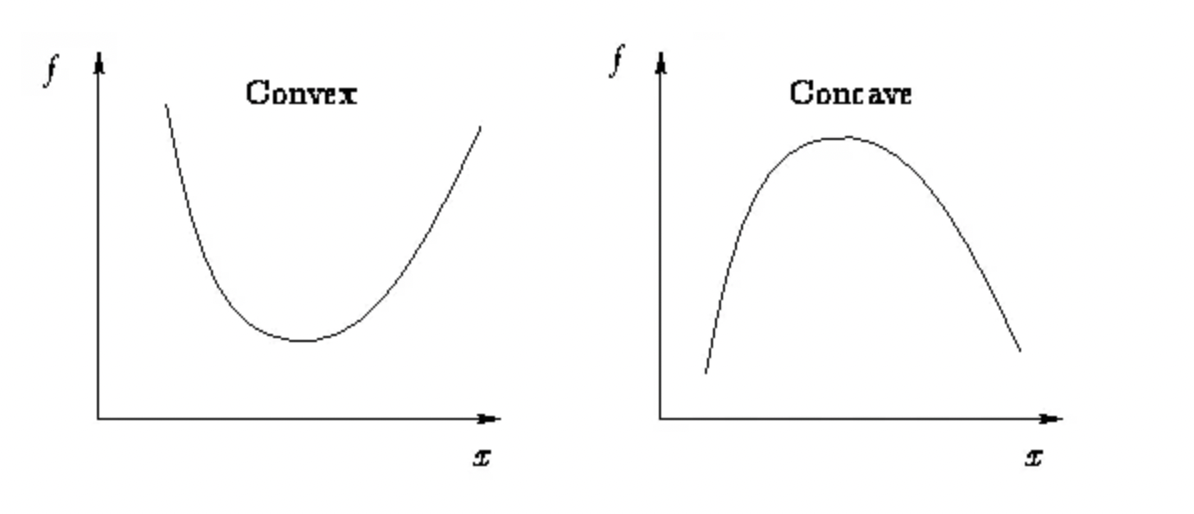
\includegraphics[width=0.5\textwidth]{Screen Shot 2023-09-18 at 10.38.18 AM.png}
    % \caption{convex and concave }
    % \label{fig:sample}
\end{figure}

\begin{align*}
    Y = f(x) 
\end{align*}

Note: $F(x)$ is $R^1$ (\textit{i.e.,} 1-dimensional) because there is only one input. But we're drawing it in $R^2$ (\textit{i.e.,} 2-dimensional) because we're using an x-y graph. To visualize a $n$ dimensional function you need a $n+1$ dimensions because you need an additional dimension for the output.

\section{Quasi-Concavity/Convexity in $R^2$}

If a function is in $R^2$ (\textit{i.e.} it takes two inputs) then you must evaluate if  the function is convex or concave in $R^3$. That will determine if the function is convex or concave. But then if you graph you function in $R^2$ space (meaning you're not using an additional dimension for the output) the function may look convex or concave in the lower dimension. Despite how it looks in the lower dimension, you must determine if it's quasi-convex or quasi-concave from the higher dimension.  \\

If the function is convex in $R^3$, when you graph it in $R^2$ it's quasi-convex. If the function is concave in $R^3$, when graphed in $R^2$ it's quasi-concave. 

\section{Sequences and Series}

\textbf{Sequence:} The result of a function where the only inputs are integers. Any real number can be represented as a sequence. The output of a sequence is usually a set (or list) of numbers. \\

\textbf{Series:} A summation of a sequence. The output of a series is typically a single number. \\

\textbf{Infinity:} Arbitrarily long unit. Infinity is not a real number, it's a concept. \\

\textbf{Example one: } Consider the following sequence, 
\begin{align*}
    -1, -1/2, -1/3, -1/4, -1/5,...
\end{align*}

The limit of the sequence goes to zero 
\begin{align*}
    lim \rightarrow 0
\end{align*}

\textbf{Zero:} Zero is also a unique number because (unless you're being so careful) it can lose it's unit. If you say Eli has 6 apples, then you take 6 apples from him, you may not say Eli has zero \textit{apples}. You might instead say he has \textit{nothing} (which has no unit). \\

\textbf{Monotone:} The function is \textit{only} increasing or \textit{only} decreasing. The function is always going in the same direction of increasing or decreasing. \\

\textbf{Bound:} If the output of a function never increases above a certain number, then it is bounded from above. If it's output never decreases below a certain number, it's bounded from below. \\

\textbf{Example two:} Consider the following function 
\begin{align*}
    f(x) = -1^x\\
    \text{output: -1, 1, -1, 1, -1, 1, ... } 
\end{align*}

This is an example of a sequence that is \textit{bounded} by $-1$ and $1$. However, it has \textit{ no limit} and is \textit{not monotonic.}\\

It's important to understand bounds, limits and monotonicity so that when you collect data you can understand the general ways two things are related to one another. \\

% \textbf{Note on limits and infinity: } You cannot \textit{really} say the limit is infinity. Limits needs to be a real number and infinity is not a real number so this is sloppy notation. \\

\textbf{Method of exhaustion:} Find examples of methods of exhaustion videos and post by October 2nd. \\

\textbf{Some infinities are bigger than others:} Some infinities are \textit{countable} meaning you can write down an expression that can denote any number in your sequence. However, some infinities are not countable. \\

\textbf{Examples:}
Let $a$ be a real number, $0<a<\infty$,

\begin{align*}
    \lim_{N\to\infty} \frac{a}{N} = \infty\\
    \lim_{N\to\infty} \frac{N}{N+a} = 1\\
\end{align*}

Building intuition on a complicated limit: 
\begin{align*}
    \lim_{N \to \infty} \Bigg(1+ \frac{1}{N}\Bigg)^N  = e
\end{align*}

\begin{align*}
    N = 1 \implies 2 \\
    N = 2 \implies (1+1/2)(1+1/2) = 2.25\\
    N = 3 \implies (1+1/3)(1+1/3)(1+1/3) = 2\frac{4}{9}\\
    N \rightarrow \infty \implies e \approx 2.7182...
\end{align*}

Here we built intuition here by looking at the difference in output between N=1 and N=2, then N=2 and N=3. The difference between outputs got smaller as we moved forward, so intuited that this limit would be bounded above by \textit{something}. 

\subsection{Why do we care? Future generations}
If we think about sustainable development (non-declining welfare for future generations) then how many future generations do we actually care about?? \textit{All} of the future generations? Realistically, that's probably not true. You'd probably prefer keeping you own kids healthy more than you'd care about your great-great-great-grand kids. \\

If you don't prefer the immediate generation at least a little more than the future, you would let everyone starve today in order to save all resources for future generations. That doesn't seem right either. This gets to why we use discount rates, which we'll talk about more later in class. 

\subsection{Why do we care? Science}
The more data you have the better approximation you have of real relationships. \\

\textbf{Intermediate value theorem} tells us that we should want more data. Assuming x is continuous, we can always find another x that will help us approximate the relationship between x and y more accurately. \\

Let think about slope. Consider the funciton: 
\begin{align}
    S = F(w) 
\end{align}
The slope is 
\begin{align*}
    \frac{F(w_2) - F(w_1)}{w_2-w_1} = \frac{\Delta S}{ \Delta w}
\end{align*}
Now consider if $w_2$ is arbitrarily smaller than $w_1$. $w_2 = w_1 + \epsilon$. We can write our slope equation as 
\begin{align*}
    \frac{F(w_1 + \epsilon) - F(w_1)}{\epsilon}
\end{align*}
This is the definition of a derivative, 
\begin{align*}
    \frac{ds}{dw} \equiv \lim_{\epsilon \to \ 0} \frac{F(w_1 + \epsilon) - F(w_1)}{\epsilon}
\end{align*}



\end{document}